\documentclass{article}


\usepackage[T1]{fontenc}
\usepackage[french]{babel}

\setlength{\fboxrule}{0.1pt}
\usepackage{etoolbox}

\usepackage{./utils}
\setcounter{secnumdepth}{0}
\setupplease{Rendu projet de compilation:\\interpreteur mini-ml}
{Mouhamed DIENG et Nathan HOUALET (Groupe 23)}

\begin{document}

\maketitle

{
  \thispagestyle{empty}
  \hypersetup{linkcolor=black}
  \tableofcontents
}

% \newpage

\section{Auteurs du projet et répartition du travail}
Mouhamed s'est occupé principalement de la partie Parsing et Nathan de la partie
Typage.

\pagebreak

\stepcounter{section}
\pagebreak


\section{Réponses aux questions de chaque partie du projet}

\subsection{3.1 Parseur simple : compréhension}

\question{
  Donnez l'automate LR0 associé à la grammaire ci-dessus (on considèrera
  pour cette question que built\_in, INT et ID sont un seul terminal (qu'on
  notera T), car le phénomène à observer ne les concerne pas vraiment).
  Vous pouvez évidemment vous servir de menhir pour vérifier que vous avez le
  bon automate. La grammaire simplifiée est donc la suivante (il faut évidemment
  ajouter le non-terminal initial technique expr' pour avoir un résultat
  similaire à menhir)
}{
  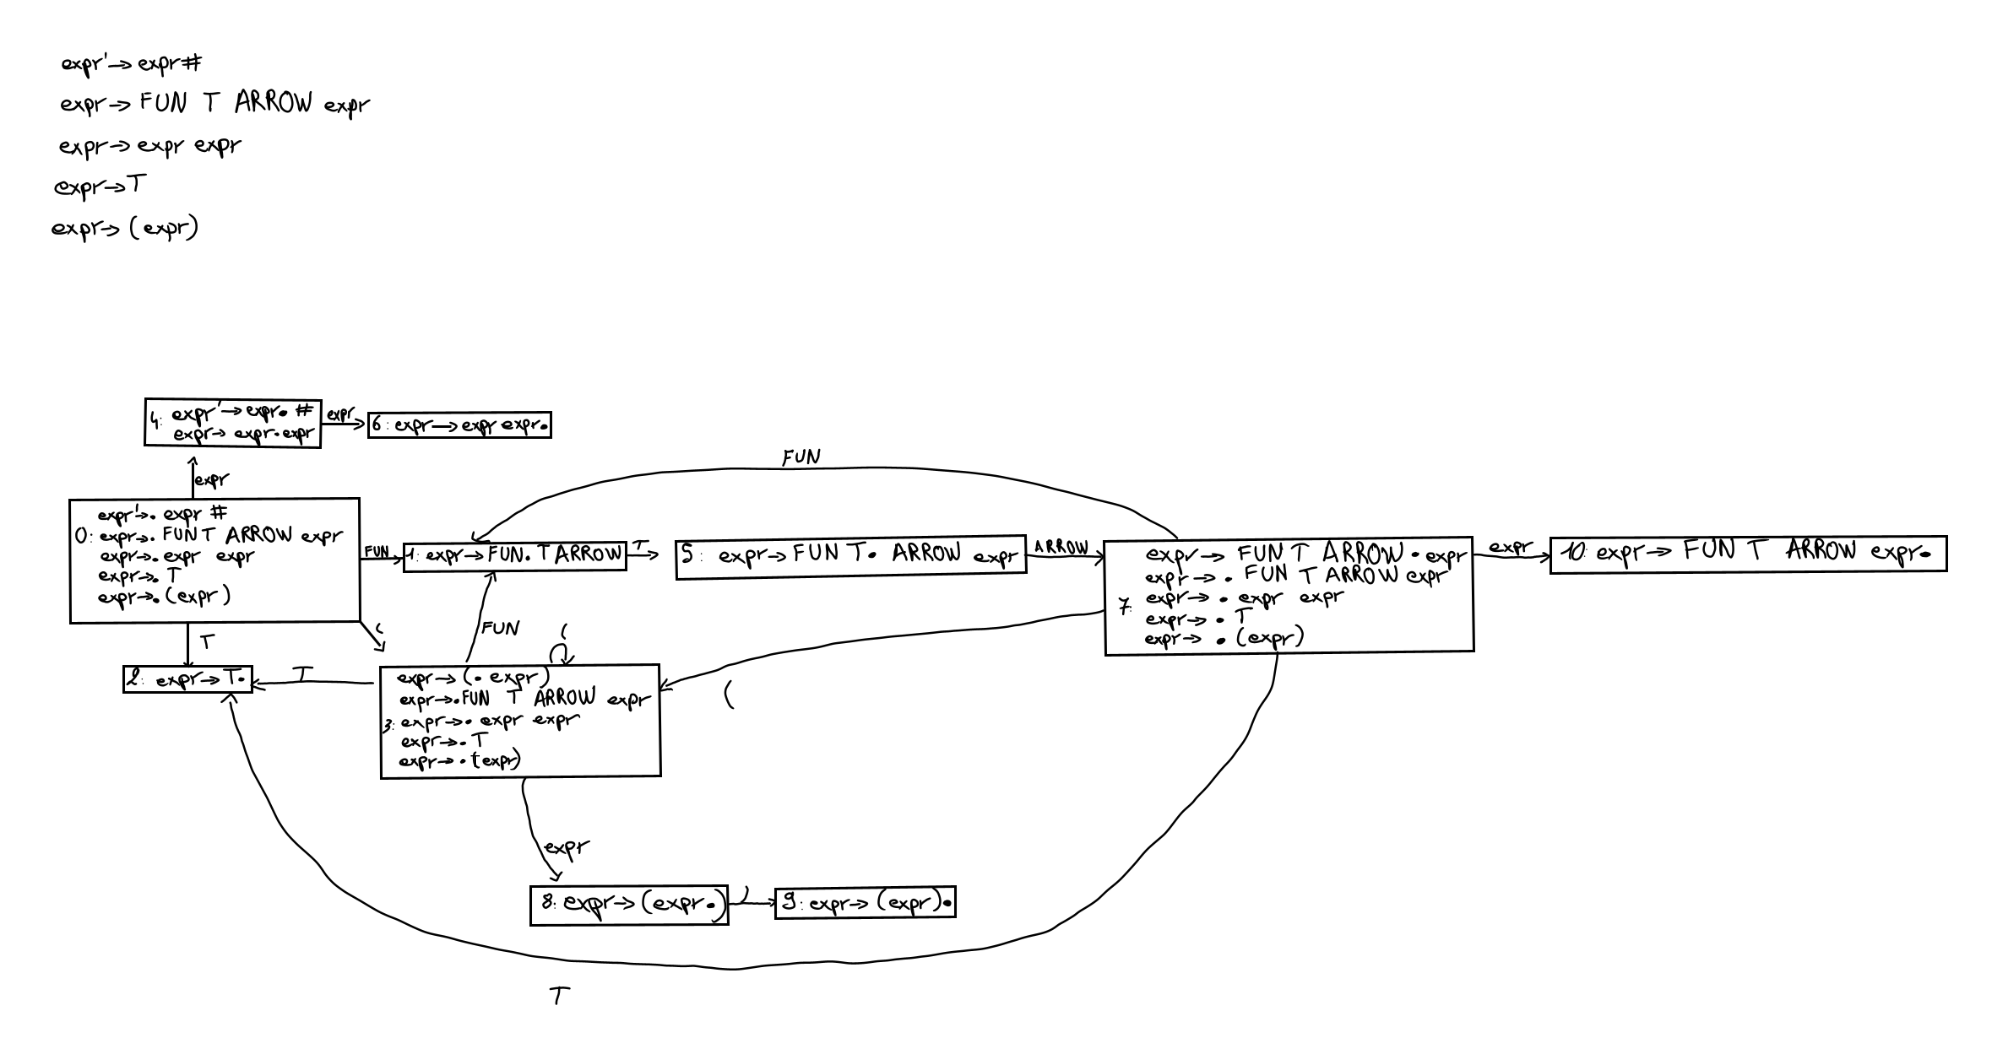
\includegraphics[width=0.95\textwidth,height=\textheight,keepaspectratio]
  {./assets/3_1_automate.png} 
}
{}

\question{
  Où sont les conflits sur cet automate, si on le considère comme un automate
  SLR ?
}
{
  Follow(expr) = \{ \#, FUN, T , ( , ) \}
  \\
  Si on considère l'automate comme un automate SLR, les conflits sont dans les 
  états 2, 6 et 10.
}
{}

\question{
  Donnez un exemple de séquence de tokens sur laquelle deux arbres de
  dérivations sont possibles avec cet automate. Qu'en déduisez-vous sur cette
  grammaire naturelle ?
}
{
  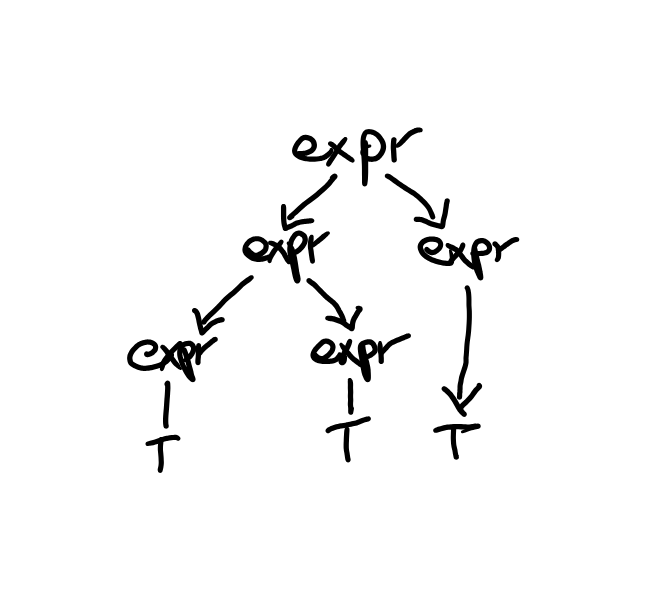
\includegraphics[width=0.35\textwidth,height=\textheight,keepaspectratio]
  {./assets/TTT_left.png} 
  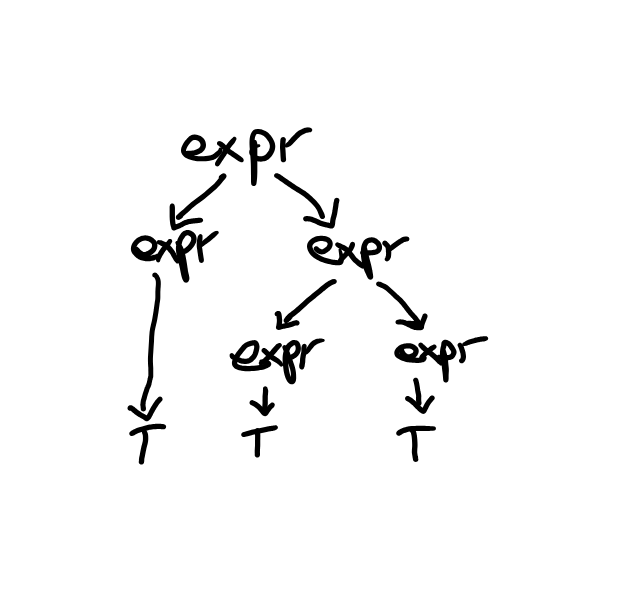
\includegraphics[width=0.35\textwidth,height=\textheight,keepaspectratio]
  {./assets/TTT_right.png}
  \\
  Pour la séquence TTT, il existe plusieurs arbres de dérivation possibles,
  donc la grammaire est ambiguë.
}
{}

\question{
  Quel est le choix fait par le parseur implémenté dans Parser calc.mly
  sur votre séquence de tokens ?
}
{
  L'abre est associatif à gauche.
}
{}


\question{
  Quelles priorités peut-on ajouter à la grammaire ci-dessus pour retrouver
  le comportement de Parser calc.mly (utilisez menhir pour vérifier que vous
  avez la bonne réponse).
}
{
  On peut ajouter "\%left T"
}
{}


\question{
  Si on ajoute toutes les fonctions built\_in dans le parseur, qu'est-ce que
  cela donne en terme du nombre de priorités à écrire.
}
{
  On doit aussi mettre des priorités pour toutes les fonctions built\_in.
}
{}

\question{
  A votre avis, pourquoi donc utilisons-nous plutôt des non-terminaux
  distincts dans ce cas plutôt que des priorités ?
}
{
  Pour rendre la grammaire plus facile à comprendre et à maintenir.
}
{}

\subsection{3.2 Syntaxe étendue}

% > Vous expliquerez dans le document de réponses pour chaque point la solution
% > que vous avez adopté pour le traiter, ainsi que les éventuelles difficultés
% > rencontrées (i.e., qu'est-ce qui ne fonctionne pas correctement). Si vous
% > n'arrivez pas à traiter un des points, fournissez un exemple de programme
% > étant correctement parsé avec notre version et pas avec la vôtre.

% > Evidemment, nous n'avons listé que les priorités des opérateurs. Vous
% > expliquerez comment elles se comparent aux priorités déjà présentes dans le
% > parseur simple et pourquoi c'est cette solution qui est la bonne.

\subsection{4.1 Typage naïf et génération des contraintes}

\question{
  Implémentez la fonction type\_of\_built\_in du fichier typer util.ml 
  (attention à correctement attribuer les types universels génériques).
}
{
  L'implémentation est dans le fichier typer\_util.ml.\\
}
{}

% > **[DONE?]**
\question{
  Implémentez la fonction type\_expr du fichier typer naive.ml.
}
{
  L'implémentation est dans le fichier typer\_naive.ml.\\
}
{
  Les built\_in 'Leq' et 'Geq' sont de type 'a -> 'a -> bool. 
  Sachant que les built\_in pour les
  opération arithmetiques marche que sur des int, c'est surprenant que ces deux 
  là ne suivent pas la même logique.
}

\question{
  Donnez 3 (ou plus) petits programmes mini-ml qui illustrent le fonctionnement
  de votre typeur naïf (toutes les sous-expressions doivent être représentées).
  Vous placerez ces programmes dans examples/answers, et expliquerez ce qu'ils
  illustrent (en commentaire de ces programmes, et dans votre rapport).
}
{}
{}

\question{
  Choisissez l'un de ces programmes, et illustrez le fonctionnement du typeur
  sur celui-ci sur papier. Dessinez l'arbre, et pour chaque nœud, donnez son
  type et dites quelles contraintes ce nœud introduit (évidemment, choisissez un
  exemples où il y a des contraintes).
}
{}
{}

\question{
  Si vous avez une différence entre votre typeur et le nôtre sur l'un de vos
  programmes ou l'un des nôtres, décrivez cette différence, et expliquez d'où
  vous pensez qu'elle vient.
}
{
  Notre typeur n'assigne les contraintes dans le même ordre. Ça ne 
  devrais pas engendrer de problèmes lors de la résolution cependant. toutes les
  contraintes sont bien là, juste pas dans le même ordre.
}
{}

\subsection{4.2 Résolution des contraintes et polymorphisme faible}

\question{
  Dans les exemples de la question précédente, lesquels sont typés correctement,
  lesquels ne le sont pas ? Expliquez pourquoi.
}
{}
{}

\question{
  Observez que l'exemple donné en début de chapitre n'est pas typé. Donnez les
  parties typées, et expliquez où se situe l'erreur.
}
{
  On a:\\
  f : 'b -> 'b  , constraints : []\\
  a : 'e        , constraints : [,'b -> 'b = 'd -> 'e,'d = int]\\
  b : 'h        , constraints : [,'b -> 'b = 'g -> 'h,'g = string]\\

  - Donc avec le typeur naif:\\
  Les contraintes de a font que 'b doit être de type int et celles de b font que
  'b doit être de type string. On ne peut pas être à la fois de type int et
  string, donc le typeur renvoie une erreur (l'erreur apparait lors du typage de b).

  - Mais avec le typeur fortement polymorphe:\\
  Il n'y a pas d'erreur (on a f: 'a -> 'a, a: int, b: string)\\
  La résolution des contraintes a pu se faire correctement parce que f est 
  instancié une fois pour chaque let (c'est le premier "•" de la partie 4.3).
  Dans le "let a" f est instancié puis devient int -> int et dans le "let b" f est 
  encore instancié et devient string -> string.

}
{}

\question{
  Proposez un autre programme qui n'est pas correctement typé alors que OCaml le
  type, et expliquez pourquoi. Vous le placerez dans examples/answers.
}
{}
{}

\subsection{4.3 Typage fortement polymorphe}

\question{
  Illustrez le fonctionnement du typage polymorphe en fournissant deux exemples
  supplémentaires qui typent différemment avec les deux algorithmes de typage.
  Choisissez-en un dont vous expliquerez soigneusement où se situe la différence
  (i.e., décrivez l'application des deux algorithmes à cet exemple). Vous les
  placerez dans examples/answers.
}
{}
{}

\question{
  Si vous avez des différence entre votre implémentation et le comportement de
  l'outil qui vous est fourni, décrivez-les, et dites d'où vous pensez qu'elles
  viennent.
}
{}
{}

\subsection{5 Extensions }
«On évaluera plus favorablement un projet qui s'est concentré sur quelques-uns
des points à traiter, mais les a correctement réalisé et expliqué, qu'un
projet qui s'est dispersé et a tout mal fait.»
\\
\\
Nous n'avons pas implémenté d'extensions.

\end{document}
